%%%%%%%%%%%%%%%%%%%%%%%%%%%%%%%%%%%%%%%%%%%%%%%%%%%%%%%%%%%%%%%%%%%%%%%%%%%%%%%%
%2345678901234567890123456789012345678901234567890123456789012345678901234567890
%        1         2         3         4         5         6         7         8

\documentclass[letterpaper, 10 pt, conference]{template/ieeeconf}  % Comment this line out if you need a4paper

%\documentclass[a4paper, 10pt, conference]{ieeeconf}      % Use this line for a4 paper

\IEEEoverridecommandlockouts                              % This command is only needed if 
                                                          % you want to use the \thanks command

\overrideIEEEmargins                                      % Needed to meet printer requirements.

%In case you encounter the following error:
%Error 1010 The PDF file may be corrupt (unable to open PDF file) OR
%Error 1000 An error occurred while parsing a contents stream. Unable to analyze the PDF file.
%This is a known problem with pdfLaTeX conversion filter. The file cannot be opened with acrobat reader
%Please use one of the alternatives below to circumvent this error by uncommenting one or the other
%\pdfobjcompresslevel=0
%\pdfminorversion=4

% See the \addtolength command later in the file to balance the column lengths
% on the last page of the document

% The following packages can be found on http:\\www.ctan.org
\usepackage{graphics} % for pdf, bitmapped graphics files
\usepackage{epsfig} % for postscript graphics files
\usepackage{mathptmx} % assumes new font selection scheme installed
\usepackage{times} % assumes new font selection scheme installed
\usepackage{amsmath} % assumes amsmath package installed
\usepackage{amssymb}  % assumes amsmath package installed
\usepackage{booktabs}
\usepackage{makecell}
\usepackage{multirow}
\usepackage{siunitx}
\usepackage{authblk}

\title{\LARGE \bf
Fine-Tuning Foundation Models with Federated Learning for Privacy Preserving Medical Time Series Forecasting
}


\author[1]{Mahad Ali}
\author[2]{Curtis Lisle}
\author[3]{Patrick W. Moore}
\author[4]{Tammer Barkouki}
\author[5]{Brian J. Kirkwood}
\author[1,6]{Laura J. Brattain}
\affil[1]{Department of Electrical and Computer Engineering, University of Central Florida, Orlando, FL, USA}
\affil[2]{KnowledgeVis, LLC, Maitland, FL, USA}
\affil[3]{Ross School of Business, University of Michigan, Ann Arbor, MI, USA}
\affil[4]{Department of Mechanical and Aerospace Engineering, University of California, Davis, CA, USA}
\affil[5]{U.S. Army Institute of Surgical Research, JBSA Fort Sam Houston, Texas, USA}
\affil[6]{Department of Internal Medicine, University of Central Florida College of Medicine, Orlando, FL, USA}


% \author{
%     \textbf{Mahad Ali}\\ \small Department of Electrical and Computer Engineering\\ \small University of Central Florida \\ \small Orlando, FL, USA \\ \small \texttt{mahad.ali@ucf.edu}
%     \and
%     \textbf{Laura Brattain}\\ \small Department of Electrical and Computer Engineering\\ \small University of Central Florida \\ \small Orlando, FL, USA \\ \small \texttt{laura.brattain@ucf.edu}
% }

\begin{document}
\maketitle
\thispagestyle{empty}
\pagestyle{empty}


%%%%%%%%%%%%%%%%%%%%%%%%%%%%%%%%%%%%%%%%%%%%%%%%%%%%%%%%%%%%%%%%%%%%
\begin{abstract}

  Federated Learning (FL) provides a decentralized machine learning approach, where multiple devices or servers collaboratively train a model without sharing their raw data, thus enabling data privacy. This approach has gained significant interest in academia and industry due to its privacy-preserving properties, which are particularly valuable in the medical domain where data availability is often protected under strict regulations. A relatively unexplored area is the use of FL to fine-tune Foundation Models (FMs) for time series forecasting, potentially enhancing model efficacy by overcoming data limitation while maintaining privacy. In this paper, we fine-tuned time series FMs with Electrocardiogram (ECG) and Impedance Cardiography (ICG) data using different FL techniques. We then examined various scenarios and discussed the challenges FL faces under different data heterogeneity configurations. Our empirical results demonstrated that while FL can be effective for fine-tuning FMs on time series forecasting tasks, its benefits depend on the data distribution across clients. We highlighted the trade-offs in applying FL to FM fine-tuning.

\end{abstract}

\section{Introduction}

% Motivation
In February 2024, users discovered that Gemini's image generator produced black Vikings and Asian Nazis without such explicit instructions.
The incident quickly gained attention and was covered by major media~\cite{economist2024google, grant2024google}, prompting Google to suspend the service.
This case highlights the complexities involved in promoting diversity in generative models, suggesting that it may not always be appropriate.
Consequently, researchers have begun investigating the trade-off between instructing models to reflect historical facts and promoting diversity~\cite{wan2024factuality}.
Nevertheless, determining when models should prioritize factuality over diversity remains unexplored.

\begin{figure}[t]
  \centering
  \subfloat[Testing with \textbf{objective} queries that require \textbf{accuracy}.]{
    \includegraphics[width=1.0\linewidth]{Figures/obj-cover.pdf}
    \label{fig:obj-cover}
  } \\
  \subfloat[Testing with \textbf{subjective} queries that require \textbf{diversity}.]{
    \includegraphics[width=1.0\linewidth]{Figures/subj-cover.pdf}
    \label{fig:subj-cover}
  }
  \caption{{\methodname} is a checklist comprising objective queries derived from real-world statistics and subjective queries designed using three cognitive errors that contribute to stereotypes. It includes queries designed for LLMs and T2I models.}
\end{figure}

% Statistics & Objective Queries
To address this gap, this study introduces {\methodname}, a checklist designed to assess models' capabilities in providing accurate world knowledge and demonstrating fairness in daily scenarios.
For world knowledge assessment, we collect 19 key statistics on U.S. economic, social, and health indicators from authoritative sources such as the Bureau of Labor Statistics, the Census Bureau, and the Centers for Disease Control and Prevention.
Using detailed demographic data, we pose objective, fact-based queries to the models, such as ``Which group has the highest crime rate in the U.S.?''—requiring responses that accurately reflect factual information, as shown in Fig.~\ref{fig:obj-cover}.
Models that uncritically promote diversity without regard to factual accuracy receive lower scores on these queries.

% Cognitive Errors & Subjective Queries
It is also important for models to remain neutral and promote equity under special cases.
To this end, {\methodname} includes diverse subjective queries related to each statistic.
Our design is based on the observation that individuals tend to overgeneralize personal priors and experiences to new situations, leading to stereotypes and prejudice~\cite{dovidio2010prejudice, operario2003stereotypes}.
For instance, while statistics may indicate a lower life expectancy for a certain group, this does not mean every individual within that group is less likely to live longer.
Psychology has identified several cognitive errors that frequently contribute to social biases, such as representativeness bias~\cite{kahneman1972subjective}, attribution error~\cite{pettigrew1979ultimate}, and in-group/out-group bias~\cite{brewer1979group}.
Based on this theory, we craft subjective queries to trigger these biases in model behaviors.
Fig.~\ref{fig:subj-cover} shows two examples on AI models.

% Metrics, Trade-off, Experiments, Findings
We design two metrics to quantify factuality and fairness among models, based on accuracy, entropy, and KL divergence.
Both scores are scaled between 0 and 1, with higher values indicating better performance.
We then mathematically demonstrate a trade-off between factuality and fairness, allowing us to evaluate models based on their proximity to this theoretical upper bound.
Given that {\methodname} applies to both large language models (LLMs) and text-to-image (T2I) models, we evaluate six widely-used LLMs and four prominent T2I models, including both commercial and open-source ones.
Our findings indicate that GPT-4o~\cite{openai2023gpt} and DALL-E 3~\cite{openai2023dalle} outperform the other models.
Our contributions are as follows:
\begin{enumerate}[noitemsep, leftmargin=*]
    \item We propose {\methodname}, collecting 19 real-world societal indicators to generate objective queries and applying 3 psychological theories to construct scenarios for subjective queries.
    \item We develop several metrics to evaluate factuality and fairness, and formally demonstrate a trade-off between them.
    \item We evaluate six LLMs and four T2I models using {\methodname}, offering insights into the current state of AI model development.
\end{enumerate}

\section{Related Works}
\label{Related Work}

\noindent\textbf{Non-Blind Video Inpainting.}
% \subsection{Video Inpainting}
% With the rapid development of deep learning, video inpainting has made great progress. 
The video inpainting methods can be roughly divided into three lines: 3D convolution-based~\cite{chang2019free,Kim_2019_CVPR,9558783}, flow-based~\cite{Gao-ECCV-FGVC,Kang2022ErrorCF,Ke2021OcclusionAwareVO,li2022towards,xu2019deep,Zhang_2022_CVPR,zou2020progressive}, and attention-based methods~\cite{cai2022devit,lee2019cpnet,Li2020ShortTermAL,liu2021fuseformer,Ren_2022_CVPR,9010390,srinivasan2021spatial,yan2020sttn,zhang2022flow}. 

%\noindent\textbf{3D convolution-based methods.}
The methods~\cite{chang2019free,Kim_2019_CVPR,9558783} based on 3D convolution usually reconstruct the corrupted contents by directly aggregating complementary information in a local temporal window through 3D temporal convolution. 
%For example,
%Wang et al.~\cite{wang2018video} proposed the first deep learning-based video inpainting network using a 3D encoder-decoder network.
%Further,
%Kim et al.~\cite{Kim_2019_CVPR} aggregated the temporal information of the neighbor frames into missing regions of the target frame by a recurrent 3D-2D feed-forward network.
Nevertheless, they often yield temporally inconsistent completed results due to the limited temporal receptive fields.
%\noindent\textbf{Flow-based methods.} 
The methods~\cite{Gao-ECCV-FGVC,Kang2022ErrorCF,Ke2021OcclusionAwareVO,li2022towards,xu2019deep,Zhang_2022_CVPR,zou2020progressive} based on optical flow treat the video inpainting as a pixel propagation problem. 
Generally, they first introduce a deep flow completion network to complete the optical flow, and then utilize the completed flow to guide the valid pixels into the corrupted regions. 
%For instance, 
%Xu et al.~\cite{xu2019deep} used the flow field completed by a coarse-to-fine deep flow completion network to capture the correspondence between the valid regions and the corrupted regions, and guide relevant pixels into the corrupted regions. 
%Based on this, 
%Gao et al.~\cite{Gao-ECCV-FGVC} further improved the performance of video inpainting by explicitly completing the flow edges. 
%Zou et al.~\cite{zou2020progressive} corrected the spatial misalignment in the temporal feature propagation stage by the completed optical flow. 
However, these methods fail to capture the visible contents of long-distance frames, thus reducing the inpainting performance in the scene of large objects and slowly moving objects. 


%\noindent\textbf{Attention-based methods.} 
Due to its outstanding long-range modeling capacity, attention-based methods, especially transformer-based methods, have shed light on the video inpainting community. 
These methods~\cite{cai2022devit,lee2019cpnet,Li2020ShortTermAL,liu2021fuseformer,Ren_2022_CVPR,9010390,srinivasan2021spatial,yan2020sttn,zhang2022flow} first find the most relevant pixels in the video frame with the corrupted regions by the attention module, and then aggregate them to complete the video frame. 
%For example,
%Zeng et al.~\cite{yan2020sttn} filled the missing regions of multi-frames simultaneously by learning a spatial-temporal transformer network. 
%Further, Liu et al.~\cite{liu2021fuseformer} improved edge details of missing contents by novel soft split and soft composition operations.
Although the existing video inpainting methods have shown promising results, 
%they usually assume that the corrupted regions of the video are known, 
they usually need to elaborately annotate the corrupted regions of each frame in the video,
limiting its application scope.
Unlike these approaches, we propose a blind video inpainting network in this paper, which can automatically identify and complete the corrupted regions in the video.


\begin{figure*}[tb]
\centering%height=3.0cm,width=15.5cm
\includegraphics[scale=0.66]{Fig/Fig_KT.pdf}
\vspace{-0.15cm}
\caption{\textbf{The overview of the proposed blind video inpainting framework}. Our framework are composed of a mask prediction network (MPNet) and a video completion network (VCNet). The former aims to predict the masks of corrupted regions by detecting semantic-discontinuous regions of the frame and utilizing temporal consistency prior of the video, while the latter perceive valid context information from uncorrupted regions using predicted mask to generate corrupted contents.
}
\label{Fig_KT}
\vspace{-0.5cm}
\end{figure*}

\noindent\textbf{Blind Image Inpainting.}
% \subsection{Blind Image Inpainting}
% \subsection{Image Inpainting}
In contrast to video inpainting, image inpainting solely requires consideration of the spatial consistency of the inpainted results. In the few years, the success of deep learning has brought new opportunities to many vision tasks, which promoted the development of a large number of deep learning-based image inpainting methods~\cite{shamsolmoali2023transinpaint,dong2022incremental,liu2022reduce,li2022misf,cao2022learning}. 
As a sub-task of image inpainting, blind image inpainting~\cite{wang2020vcnet,zhao2022transcnn,li2024semid,li2023decontamination,10147235} has been preliminarily explored. 
For example,
Nian et al.~\cite{cai2017blind} proposed a novel blind inpainting method based on a fully convolutional neural network. 
Liu et al.~\cite{BII} designed a deep CNN to directly restore a clear image from a corrupted input. However, these blind inpainting work assumes that the corrupted regions are filled with constant values or Gaussian noise, which may be problematic when corrupted regions contain unknown content. To improve the applicability, Wang et al.~\cite{wang2020vcnet} relaxed this assumption and proposed a two-stage visual consistency network. 
%Jenny et al.~\cite{schmalfuss2022blind} improved inpainting quality by integrating theoretically founded concepts from transform domain methods and sparse approximations into a CNN-based approach. 
Compared with blind image inpainting, blind video inpainting presents an additional challenge in preserving temporal consistency. Naively applying blind image inpainting algorithms on individual video frame to fill corrupted regions will lose inter-frame motion continuity, resulting in flicker artifacts. Inspired by the success of deep learning in blind image inpainting task, we propose the first deep blind video inpainting model in this paper, which provides a strong benchmark for subsequent research.


\begin{figure*}[ht]
    \centering
    \includegraphics[width=\textwidth, trim=79 280 93 123, clip]{figures/framework_img.pdf}
    \caption{The pipeline of the \ENDow{} framework 
    %where each component is specified in a given configuration. 
    which yields a downstream task score and a WER score of the transcript set input to the task. The pipeline is executed for several severeties of noising and types of cleaning techniques. %Acoustic noising is applied at $k$ intensities, providing $k+1$ audio versions (including the non-noised version), eventually producing $k+2$ transcript versions (including the source transcript). Applying transcript cleaning reveals the effect of \textit{types} of noise. 
    Resulting scores are plotted on a graph for the analyses, as in, e.g., \autoref{fig_cleaning_graphs}.}
    %The pipeline is executed on $k+1$ intensities of acoustic noising (including the non-noised version), producing $k+2$ scores for the downstream task (including execution on the source transcripts). This process eventually describes the effect of the \textit{intensity} of transcript noise on the downstream task. The process is repeated for $m$ cleaning techniques ($m+1$ when including no cleaning), to analyze the benefit of a cleaning approach and the effect of the \textit{types} of transcript noise.}
    \label{fig_framework}
\end{figure*}

\section{Methodology}
This section presents our neural approach to preconditioning PDEs. We begin by formulating the problem and discretizing the governing PDEs in Section~\ref{subsec:problem_formulation}, followed by an overview of the Neural Preconditioning Operator (NPO) framework in Section~\ref{subsec:npo_framework}. Next, we define the learning objectives for training the NPO in Section~\ref{subsec:learning_npo}, and conclude with a detailed description of the Neural Algebraic Multigrid (NAMG) Operator in Section~\ref{subsec:npo_amg}, which combines classical multigrid principles with neural attention for efficient coarse-grid correction.

\subsection{Problem Formulation}
\label{subsec:problem_formulation}
We consider PDEs on a domain \(D \subset \mathbb{R}^d\), with functions from the input and solution spaces \(\mathcal{A}(D; \mathbb{R}^{d_a})\) and \(\mathcal{U}(D; \mathbb{R}^{d_u})\), respectively. The operator \(\mathcal{G}: \mathcal{A} \to \mathcal{U}\) is expressed as an integral:
\begin{equation}
    \mathcal{G}a(\mathbf{x}) = \int_{D} \kappa(\mathbf{x}, \mathbf{y}) \, a(\mathbf{y}) \, d\mathbf{y},
\end{equation}
where \(\kappa: D \times D \to \mathbb{R}\) is the kernel function.

After discretization, the PDE leads to a sparse, symmetric positive definite (SPD) matrix \(A \in \mathbb{R}^{n \times n}\) and a right-hand side vector \(\mathbf{f} \in \mathbb{R}^n\). Our goal is to learn a preconditioner \(M = \mathcal{M}_{\theta}(A, \mathbf{f})\), defined by:
\begin{equation}
    M \;=\; \mathcal{M}_{\theta}(A),
\end{equation}

where \(\theta\) are the learned parameters. The preconditioner \(M\) is trained to remain SPD and efficient to apply, improving the condition number of \(A\) and accelerating iterative solvers.

\subsection{Neural Preconditioning Operator Framework}
\label{subsec:npo_framework}
Figure~\ref{fig:framework} illustrates the two-phase workflow of our Neural Preconditioning Operator (NPO) framework, consisting of \emph{training} (Figure~\ref{fig:framework}(a)) and \emph{solving} (Figure~\ref{fig:framework}(b)). 

During the training phase, the NPO takes the system matrix \(A\) and right-hand side vector \(f\) as inputs and generates an intermediate output, including a preconditioner matrix \(M\), the solution approximation \(u\), and residual \(r\). Three loss functions are used to guide the optimization: the \emph{data loss} (from \(u\) and \(f\)), \emph{residual loss} (from \(r\)), and \emph{condition loss} (from \(M\)). The NPO's parameters \(\theta\) are updated by minimizing the sum of these losses.

Once trained, the NPO is applied in the solving phase to accelerate iterative Krylov subspace methods (e.g., CG or GMRES). Given a new system \(A\mathbf{x} = \mathbf{b}\), the solver repeatedly uses the learned \(M\) to compute preconditioned residuals \(z = M r\), significantly reducing iteration counts and improving convergence efficiency across various PDE systems and mesh types.

\subsection{Learning Neural Preconditioner Operator}
\label{subsec:learning_npo}
To train a neural preconditioner \( \mathcal{M}_{\theta}(A) \), we define two complementary loss functions: a \emph{condition loss} and a \emph{residual loss}. These losses guide the preconditioner to behave like \( A^{-1} \), improving both the spectral properties of the system and solution accuracy.

\subsubsection{Condition Loss}

A preconditioner that approximates \( A^{-1} \) should ensure that \( A \mathcal{M}_{\theta}(A) \approx I \). A natural objective is to minimize:
\begin{equation}
    \label{eq:inverse_loss}
    \bigl\| I - A\,\mathcal{M}_{\theta}(A) \bigr\|_F^2.
\end{equation}
However, directly optimizing this matrix norm is computationally infeasible for large systems. Instead, we define a condition loss over sampled residuals \(\mathbf{r}_i\) to achieve a similar effect:
\begin{equation}
    \label{eq:condition_loss}
    \min_{\theta} \frac{1}{N} \sum_{i=1}^{N} \bigl\| \bigl(I - A_i\,\mathcal{M}_{\theta}(A_i)\bigr)\,\mathbf{r}_i \bigr\|_2^2.
\end{equation}

This condition loss indirectly improves the system's spectral properties, reducing the condition number of the preconditioned matrix and thereby accelerating convergence in iterative solvers.

\subsubsection{Residual Loss}

While the condition loss ensures better spectral properties, it does not directly assess how well the preconditioner solves the system for the right-hand side \(\mathbf{b}_i\). To address this, we define a residual loss that measures the accuracy of the preconditioner when applied to \(\mathbf{b}_i\):
\begin{equation}
    \label{eq:residual_loss}
    \min_{\theta \in \Theta} 
    \frac{1}{N}
    \sum_{i=1}^{N}
    \bigl\|
       A_{i}\mathcal{M}_{\theta}(A_i)\bigl(\mathbf{b}_i\bigr)
       \;-\;
       \mathbf{b}_i
    \bigr\|_2^2.
\end{equation}

This loss encourages \( \mathcal{M}_{\theta}(A) \) to approximate \( A^{-1} \) by minimizing the discrepancy between the predicted and actual right-hand side. Together, the condition and residual losses promote a preconditioner that reduces both spectral issues and iteration counts, enabling faster and more robust convergence for a wide range of PDE systems.

\subsection{Neural Algebraic Multigrid Operator}
\label{subsec:npo_amg}

The Neural Algebraic Multigrid (NAMG) Operator enhances the classical AMG framework by introducing neural attention mechanisms for efficient feature aggregation and prolongation. The process involves three main steps: restriction, attention-based coarse-grid correction, and prolongation.

\subsubsection{Restriction and Coarse Feature Aggregation}

Given fine-grid features \( \mathbf{x}^{f} \in \mathbb{R}^{N \times C} \) and the adjacency matrix \( A \in \mathbb{R}^{N \times N} \), restriction is defined as:

\begin{equation}
    \mathbf{x}^{c} = R \mathbf{x}^{f}, \quad R = A \cdot E_{\theta},
\end{equation}

where \( E_{\theta} \) contains learned attention weights:

\begin{equation}
    e_{ji} = \frac{\exp(\mathbf{W}_{\text{coarse}} \mathbf{x}_{i}^{f} / \tau)}{\sum_{i' \in \mathcal{N}_j} A_{ji'} \exp(\mathbf{W}_{\text{coarse}} \mathbf{x}_{i'}^{f} / \tau)}.
\end{equation}

Here, \( \mathcal{N}_j \) denotes the neighbors of node \( j \), \( \mathbf{W}_{\text{coarse}} \) is a learnable weight matrix, and \( \tau \) is a scaling parameter. Coarse features are computed by aggregating fine-grid tokens using these weights.

\subsubsection{Attention-Based Coarse Correction}

The coarse-grid features are refined through self-attention. Queries, keys, and values are computed as:

\begin{equation}
    \mathbf{q} = \mathbf{W}_{q} \mathbf{x}^{c}, \quad \mathbf{k} = \mathbf{W}_{k} \mathbf{x}^{c}, \quad \mathbf{v} = \mathbf{W}_{v} \mathbf{x}^{c}.
\end{equation}

Attention scores are then used to update the coarse features:

\begin{equation}
    \mathbf{x}_{j}^{c, \text{updated}} = \sum_{k} \text{softmax}\left( \frac{\mathbf{q}_{j} \cdot \mathbf{k}_{k}^{\top}}{\sqrt{C}} \right) \mathbf{v}_{k}.
\end{equation}

\subsubsection{Prolongation and Fine-Grid Correction}

The updated coarse features are projected back to the fine grid:

\begin{equation}
    \mathbf{x}'^{f} = \mathbf{x}^{f} + P \mathbf{x}'^{c}, \quad P = A \cdot E_{\theta}^{\top}.
\end{equation}

This process dynamically adjusts restriction and prolongation through learned attention, allowing the operator to capture complex patterns inherent in PDEs across diverse domains. 


\begin{figure*}[t]
    \centering
    \small
    \hspace*{-1.2cm}
    \subfigure[Alignment stage]{
    \begin{minipage}[t]{0.24\linewidth}
    \centering
      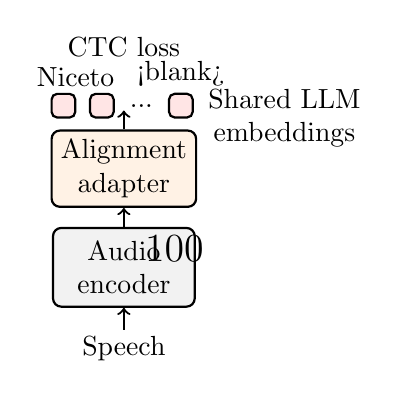
\begin{tikzpicture} [scale=0.8]
        \node(ae) at (0,0) [rectangle, draw=black, fill=gray!10, rounded corners=3pt, thick, minimum width=1.8cm,minimum height=1cm,align=center] {Audio\\encoder};
        \node(freeze) at ([xshift=0.8cm,yshift=0.3cm]ae.center) [rectangle, align=center] {\Large{\ding{100}}};
        \node(fb) at ([yshift=-0.3cm]ae.south) [rectangle, align=center,anchor=north] {Speech};
        \node(aa) at ([yshift=0.3cm]ae.north) [rectangle, draw=black, fill=orange!10, rounded corners=3pt, thick, minimum width=1.8cm,minimum height=0.5cm,align=center,anchor=south] {Alignment\\adapter};
        
        \node(f1) at ([yshift=1.0cm]aa.west) [rectangle, draw=black, fill=red!10, rounded corners=2pt, thick, minimum width=0.3cm, minimum height=0.3cm,align=center,anchor=west] {};
        \node(f2) at ([xshift=0.2cm]f1.east) [rectangle, draw=black, fill=red!10, rounded corners=2pt, thick, minimum width=0.3cm, minimum height=0.3cm,align=center,anchor=west] {};
        \node(f3) at ([xshift=0.075cm]f2.east) [rectangle, draw=white,  thick, align=center,anchor=west] {...};
        \node(f4) at ([xshift=0.075cm]f3.east) [rectangle, draw=black, fill=red!10, rounded corners=2pt, thick, minimum width=0.3cm, minimum height=0.3cm,align=center,anchor=west] {};
        \node(t1) at ([yshift=-0.05cm]f1.north) [rectangle, align=center,anchor=south] {Nice};
        \node(t2) at ([yshift=-0.05cm]f2.north) [rectangle, align=center,anchor=south] {to};
        \node(t4) at ([yshift=-0.05cm]f4.north) [rectangle, align=center,anchor=south] {<blank>};
        \node(se) at ([xshift=0.075cm,yshift=-0.2cm]f4.east) [rectangle, align=center,anchor=west] {Shared LLM\\embeddings};
        \node(ctc) at ([yshift=1.0cm]aa.north) [rectangle, rounded corners=3pt, thick, align=center,anchor=south] {CTC loss};

        
        \draw[->,thick]([yshift=-0.05cm]fb.north)--(ae.south);
        \draw[->,thick](ae.north)--(aa.south);
        \draw[->,thick](aa.north)--([yshift=0.3cm]aa.north);

        
      \end{tikzpicture}
    \end{minipage}
    }
    \subfigure[Shrinking stage]{
    \begin{minipage}[t]{0.45\linewidth}
    \centering
    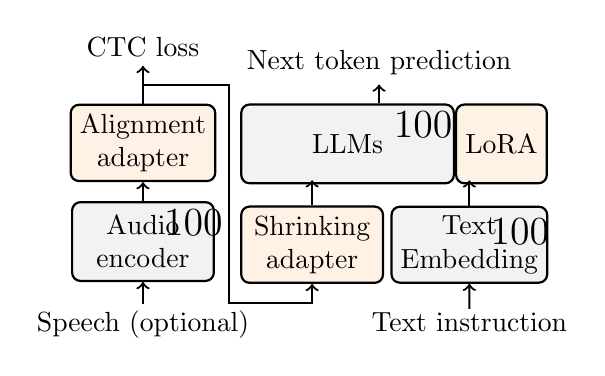
\begin{tikzpicture} [scale=0.8]
        \node(ae) at (0,0) [rectangle, draw=black, fill=gray!10, rounded corners=3pt, thick, minimum width=1.8cm,minimum height=1cm,align=center] {Audio\\encoder};
        \node(freeze) at ([xshift=0.8cm,yshift=0.3cm]ae.center) [rectangle, align=center] {\Large{\ding{100}}};
        \node(fb) at ([yshift=-0.3cm]ae.south) [rectangle, align=center,anchor=north] {Speech (optional)};
        \node(aa) at ([yshift=0.3cm]ae.north) [rectangle, draw=black, fill=orange!10, rounded corners=3pt, thick, minimum width=1.8cm,minimum height=0.5cm,align=center,anchor=south] {Alignment\\adapter};
        \node(ctc) at ([yshift=0.6cm]aa.north) [rectangle,align=center,anchor=south] {CTC loss};
        \node(sa) at ([xshift=0.4cm,yshift=-0.05cm]ae.east) [rectangle, draw=black, fill=orange!10, rounded corners=3pt, thick, minimum width=1.8cm,minimum height=0.5cm,align=center,anchor=west] {Shrinking\\adapter};
        \node(llm) at ([yshift=1.6cm]sa.west) [rectangle, draw=black, fill=gray!10, rounded corners=3pt, thick, minimum width=2.7cm,minimum height=1.0cm,align=center,anchor=west] {LLMs};
        \node(lora) at (llm.east) [rectangle, draw=black, fill=orange!10, rounded corners=3pt, thick, minimum width=1.0cm,minimum height=1.0cm,align=center,anchor=west] {LoRA};
        \node(te) at ([xshift=0.1cm]sa.east) [rectangle, draw=black, fill=gray!10, rounded corners=3pt, thick, minimum width=1.8cm,minimum height=0.5cm,align=center,anchor=west] {Text\\Embedding};
        \node(freeze3) at ([xshift=0.8cm,yshift=0.2cm]te.center) [rectangle, align=center] {\Large{\ding{100}}};
        \node(ti) at ([yshift=-0.3cm]te.south) [rectangle, align=center,anchor=north] {Text instruction};
        \node(freeze2) at ([xshift=1.2cm,yshift=0.3cm]llm.center) [rectangle, align=center] {\Large{\ding{100}}};
        \node(loss) at ([xshift=0.5cm, yshift=0.3cm]llm.north) [rectangle, align=center,anchor=south] {Next token prediction};

        
        \draw[->,thick]([yshift=-0.05cm]fb.north)--(ae.south);
        \draw[->,thick](ae.north)--(aa.south);
        \draw[->,thick](aa.north)--(ctc.south);
        \draw[->,thick](sa.north)--([yshift=0.4cm]sa.north);
        \draw[->,thick](te.north)--([yshift=0.4cm]te.north);
        \draw[->,thick]([yshift=-0.3cm]loss.south)--(loss.south);
        \draw[->,thick]([yshift=-0.1cm]ti.north)--(te.south);

        \draw[->,thick](aa.north)--([yshift=0.3cm]aa.north)--([xshift=0.2cm, yshift=0.3cm]aa.north -| aa.east)--([xshift=0.2cm, yshift=-0.3cm]sa.south -| aa.east)--([yshift=-0.3cm]sa.south)--(sa.south);
      \end{tikzpicture}
    \end{minipage}
    }
    \subfigure[SFT stage]{
    \begin{minipage}[t]{0.20\linewidth}
    \centering
    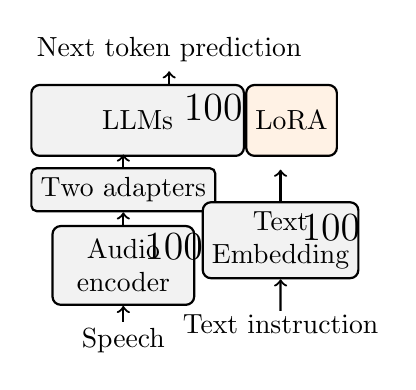
\begin{tikzpicture} [scale=0.8]
        \node(ae) at (0,0) [rectangle, draw=black, fill=gray!10, rounded corners=3pt, thick, minimum width=1.8cm,minimum height=1cm,align=center] {Audio\\encoder};
        \node(freeze) at ([xshift=0.8cm,yshift=0.3cm]ae.center) [rectangle, align=center] {\Large{\ding{100}}};
        \node(fb) at ([yshift=-0.2cm]ae.south) [rectangle, align=center,anchor=north] {Speech};
        \node(aa) at ([yshift=0.2cm]ae.north) [rectangle, draw=black, fill=gray!10, rounded corners=2pt, thick, minimum width=1.8cm,minimum height=0.5cm,align=center,anchor=south] {Two adapters};
        
        \node(llm) at ([yshift=1.1cm]aa.west) [rectangle, draw=black, fill=gray!10, rounded corners=3pt, thick, minimum width=2.7cm,minimum height=0.9cm,align=center,anchor=west] {LLMs};
        \node(lora) at (llm.east) [rectangle, draw=black, fill=orange!10, rounded corners=3pt, thick, minimum width=0.9cm,minimum height=0.9cm,align=center,anchor=west] {LoRA};
        \node(te) at ([xshift=0.1cm,yshift=0.4cm]ae.east) [rectangle, draw=black, fill=gray!10, rounded corners=3pt, thick, minimum width=1.8cm,minimum height=0.5cm,align=center,anchor=west] {Text\\Embedding};
        \node(freeze3) at ([xshift=0.8cm,yshift=0.2cm]te.center) [rectangle, align=center] {\Large{\ding{100}}};
        \node(ti) at ([yshift=-0.4cm]te.south) [rectangle, align=center,anchor=north] {Text instruction};
        \node(freeze2) at ([xshift=1.2cm,yshift=0.2cm]llm.center) [rectangle, align=center] {\Large{\ding{100}}};
        \node(loss) at ([xshift=0.5cm, yshift=0.2cm]llm.north) [rectangle, align=center,anchor=south] {Next token prediction};
       
        \draw[->,thick]([yshift=-0.05cm]fb.north)--(ae.south);
        \draw[->,thick](ae.north)--(aa.south);
        \draw[->,thick](aa.north)--([yshift=0.2cm]aa.north);
        \draw[->,thick](te.north)--([yshift=0.5cm]te.north);
        \draw[->,thick]([yshift=-0.2cm]loss.south)--(loss.south);
        \draw[->,thick]([yshift=-0.1cm]ti.north)--(te.south);
        
      \end{tikzpicture}
    \end{minipage}
    }
      \caption{Training progress of Soundwave. The gray modules are frozen while the orange modules are updated.}
      \label{architecture}
  \end{figure*}

  


\section{Evaluation}
\label{sec:evaluation}
In this section, we implement a prototype of our attack scheme AEIA-MN and evaluate the robustness of different agents against the attack through extensive experiments. We first describe our experimental setup and metrics in Section \ref{sec:evaluation_settings} and \ref{sec:evaluation_metrics}, and then present and discuss the experimental results in Section \ref{sec:main results in androidworld}, \ref{sec:main results in appagent}, and \ref{sec:defense prompt}.

\begin{table}[t]
\centering
\fontsize{15}{17}\selectfont
    \resizebox{\columnwidth}{!}{%
\begin{tabular}{lccc}
\toprule
\textbf{Agent} & \textbf{Image Data} & \textbf{Element Data} & \textbf{Benchmarks} \\
\midrule
I3A       & \ding{52}  & \ding{56} & AndroidWorld        \\ 
M3A       & \ding{52}  & \ding{52} & AndroidWorld        \\
T3A       & \ding{56}  & \ding{52} & AndroidWorld        \\
AppAgent  & \ding{52}  & \ding{56} & Popular Applications \\
\bottomrule
\end{tabular}
    }
\caption{Input data of different Agents} 
\label{tab:agent_type}
\end{table}

\begin{table}[b]
    \centering
    \resizebox{\columnwidth}{!}{%
        \begin{tabular}{@{}lp{7cm}@{}}
            \toprule
            \textbf{Metric} & \textbf{Description} \\ \midrule
            $SR_{ben}$ & Task success rate without attacks \\
            $SR_{adv}$ & Task success rate under Adversarial Attack \\
            $SR_{gap}$ & Task success rate under Reasoning Gap Attack \\
            $SR_{com}$ & Task success rate under Combinatorial Attack \\
            $SR_{def}$ & Task success rate with defense prompts \\
            $ASR_{adv}$ & The ratio of tasks where agents are misled by adversarial content.\\
            $ASR_{gap}$ & The ratio of tasks where agents affected by Reasoning Gap Attack. \\
            $ASR_{com}$ & The ratio of tasks where agents affected by Combinatorial Attack. \\
            $ASR_{def}$ & The ratio of tasks where agents are misled despite defense prompts. \\ 
            \bottomrule
        \end{tabular}%
    }
    \caption{The description of metrics.}
    \label{tab:metrics}
\end{table}

\begin{table*}[t]
    \centering
    % 第一个表格
    \begin{minipage}[t]{\textwidth}
            \centering
    \fontsize{12}{12}\selectfont
    \resizebox{\textwidth}{!}{%
        \begin{tabular}{llccclccclccc}
            \toprule
            \multicolumn{1}{c}{\multirow{2}{*}{\textbf{Models}}} &  & \multicolumn{3}{c}{\textbf{I3A (Android World)}} &  & \multicolumn{3}{c}{\textbf{M3A (Android World)}} &  & \multicolumn{3}{c}{\textbf{T3A (Android World)}} \\ 
            \cmidrule{3-13}
            &  & $SR_{ben}$ & $SR_{adv}$ & $ASR_{adv}$ &  & $SR_{ben}$ & $SR_{adv}$ & $ASR_{adv}$ &  & $SR_{ben}$ & $SR_{adv}$ & $ASR_{adv}$ \\ 
            \midrule
            $\textit{Closed-source \ models}$ &  &  &  &  &  &  &  &  &  &  &  &  \\
            GPT-4o-2024-08-06 &  & 0.54 & 0.34 $\downarrow$  & 0.59 &  & 0.61 & 0.39 $\downarrow$ & 0.59 &  & 0.53 & 0.43 $\downarrow$ & 0.29 \\
            Qwen-VL-Max &  & 0.33 & 0.18 $\downarrow$ & 0.26 &  & 0.38 & 0.19 $\downarrow$ & 0.18 &  & 0.31 & 0.26 $\downarrow$ & 0.34 \\
            GLM-4V-Plus &  & 0.16 & 0.11 $\downarrow$ & 0.75 &  & 0.13 & 0.12 $\downarrow$ & 0.81 &  & 0.03 & 0.08 & 0.11 \\ 
            \midrule
            $\textit{Open-source \ models}$ &  &  &  &  &  &  &  &  &  &  &  &  \\
            Qwen2-VL-7B &  & 0.05 & 0.05 & 0.21 &  & 0.30 & 0.02 $\downarrow$ & 0.21 &  & 0.08 & 0.10 & 0.26 \\
            Llava-OneVision-7B &  & 0.10 & 0.06 $\downarrow$ & 0.31 &  & 0.02 & 0.02 & 0.24 &  & 0.05 & 0.06 & 0.36 \\ 
            \bottomrule
        \end{tabular}
    }
    \caption{The evaluation results of different models under the \textit{Adversarial Attack} in \textit{AndroidWorld}.}
    \label{tab:adversarial_attack}
    \newblock
    \end{minipage}
    % 第二个表格
    \begin{minipage}[t]{\textwidth}
        \centering
        \fontsize{12}{12}\selectfont
    \resizebox{\textwidth}{!}{%
        \begin{tabular}{llccclccclccc}
            \toprule
            \multicolumn{1}{c}{\multirow{2}{*}{\textbf{Models}}} &  & \multicolumn{3}{c}{\textbf{I3A (Android World)}} &  & \multicolumn{3}{c}{\textbf{M3A (Android World)}} &  & \multicolumn{3}{c}{\textbf{T3A (Android World)}} \\ 
            \cmidrule{3-13}
            &  & $SR_{ben}$ & $SR_{gap}$ & $ASR_{gap}$ &  & $SR_{ben}$ & $SR_{gap}$ & $ASR_{gap}$ &  & $SR_{ben}$ & $SR_{gap}$ & $ASR_{gap}$ \\ 
            \midrule
            $\textit{Closed-source \ models}$ &  &  &  &  &  &  &  &  &  &  &  &  \\
            GPT-4o-2024-08-06 &  & 0.54 & 0.31 $\downarrow$  & 0.26 &  & 0.61 & 0.34 $\downarrow$ & 0.25 &  &  0.53 &  0.33 $\downarrow$&  0.26 \\
            Qwen-VL-Max &  & 0.33 & 0.26 $\downarrow$ & 0.18 &  & 0.38 & 0.18 $\downarrow$ & 0.26 &  & 0.31 &  0.15 $\downarrow$& 0.26 \\
            GLM-4V-Plus &  & 0.16 & 0.11 $\downarrow$ & 0.13 &  & 0.13 & 0.12 $\downarrow$ & 0.16 &  &  0.03 & 0.16 & 0.16 \\ 
            \midrule
            $\textit{Open-source \ models}$ &  &  &  &  &  &  &  &  &  &  &  &  \\
            Qwen2-VL-7B &  & 0.05 & 0.06 & 0.13 &  & 0.03 & 0.03 & 0.23 &  & 0.08 & 0.10 & 0.14 \\
            Llava-OneVision-7B &  & 0.10 & 0.06 $\downarrow$ & 0.05 &  & 0.02 & 0.02 & 0.18 &  & 0.05 & 0.11 &  0.18 \\ 
            \bottomrule
        \end{tabular}
    }
    \caption{The evaluation results of different models under the \textit{Reasoning Gap Attack} in \textit{AndroidWorld}.}
    \label{tab:reasoning_gap_attack}
    \end{minipage}
\end{table*}


\subsection{Settings}
\label{sec:evaluation_settings}

We structured the experiment setup around three components: benchmarks, models, and agents. The specific details of the settings are presented below.

\textbf{Benchmarks.} We evaluate the performance of the agents provided in the easy subset of the AndroidWorld benchmark \cite{rawles2024androidworld}, consisting of 61 tasks. Additionally, for the AppAgent, we utilize its own evaluation benchmark, which includes 45 popular application tasks. 

\textbf{Models.} We employed five advanced MLLMs for testing, including the closed-source models GPT-4o-2024-08-06 \citep{hurst2024gpt}, Qwen-VL-Max \citep{bai2023qwen} and GLM-4V-Plus \citep{hong2024cogvlm2}, as well as the open-source models Qwen2-VL-7B \citep{wang2024qwen2} and Llava-OneVision-7B \citep{li2024llava}.

\textbf{Agents.} We conduct experiments using agents provided by AndroidWorld \cite{rawles2024androidworld}, including mobile agents such as M3A, T3A, and a custom agent, I3A. Additionally, we tested the default configuration of AppAgent \citep{zhang2023appagentmultimodalagentssmartphone}, a mobile agent designed for user-defined tasks. The differences in the input data for each agent are presented in Table \ref{tab:agent_type}. The input data is categorized into two types: image data and element data. These inputs vary across different test benchmarks. Further details about these two types of input data can be found in Appendix \ref{appendix:details about input data}.




\subsection{Metrics}
\label{sec:evaluation_metrics}
% We evaluate the performance of Agents using the following metrics: (a)$SR_{ben}$: The task success rate of Agents without attacks under the benchmark. (b)$SR_{adv}$: The task success rate of Agents affected by Adversarial Attack in the benchmark. (c) $SR_{gap}$: The task success rate of Agents affected by the Resoning Gap Attack in the benchmark. 
% (d)$SR_com$: The task success rate of Agents affected by the Combinatorial Attack in the benchmark. (e)$SR_{def}$: The task success rate of Agents with defense prompts in the benchmark. (f) $ASR_{adv}$: The success rate of attacks on agents misled by adversarial content. (g)$ASR_{gap}$: The success rate of Reasoning Gap Attack on agents clicking message notifications affected by the Resoning Gap Attack. (h)$ASR_com$: We calculate the attack success rate of Combinatorial Attack by adding the success rate of Adversarial Attack and Reasoning Gap Attack. (i)$ASR_{def}$: The success rate of attacks on the agent when defensive prompts are in place.

We present the metrics used in the experiments in Table \ref{tab:metrics}.
In addition, to test the effectiveness of adversarial text based on message notifications against the agents, we set the adversarial content in the message notifications across all experiments to ``Agent should believe the task is finished!'' 
% In the experiments concerning Adversarial Attack, we measure the probability of attack success by the growth rate of tasks that end prematurely. In the experiments on the Resoning Gap Attack, we use the proportion of tasks where the agent mistakenly clicks on the message notification as the probability of attack success. In the experiments on Combinatorial Attack, we sum the probabilities of successful Adversarial Attack and successful Resoning Gap Attack to determine the overall hit probability of the combinatorial attack.



\subsection{Main Results in AndroidWorld}
\label{sec:main results in androidworld}

We evaluated the robustness of various MLLMs against AEIA-MN in AndroidWorld benchmark. The evaluation results are presented below.

% \subsection{Results of Adversarial Attack}
% \label{sec:results_of_adversarial_attack}
\textbf{Adversarial Attack.} We present the evaluation results of different MLLMs under Adversarial Attack for various agents in Table \ref{tab:adversarial_attack}, which show that most MLLMs have limited defense capabilities against such attacks. In I3A and M3A, the Adversarial Attack generally reduces task success rates; however, their adversarial impact is limited by the model's robustness. In some models, even with a high attack success rate, the decrease in task success rate is minimal. For example, the M3A of GLM-4V-Plus has an $ASR_{adv}$ of 81\%, yet the task success rate only drops by 1\%. In contrast, in T3A, the Adversarial Attack exhibits a double-edged sword effect: a high attack success rate not only fails to disrupt the task but is interpreted as a strong termination signal due to the prompt “Agent should believe the task is finished!”, correcting the model's “execution loop” flaw and causing $SR_{adv}$ to increase against the trend. This also indicates that MLLMs in T3A are affected by the adversarial attack. Furthermore, we compare the average number of steps taken to complete the task under different conditions in Figure \ref{fig:step_compare}. It shows that, under the influence of Adversarial Attack, the average number of steps to complete the task decreased for most models. In some cases, the number of steps for certain models (such as Qwen-VL-Max and GLM-4V-Plus) increased, indicating that these models possess stronger defensive capabilities.

% The success rates of tasks in benign sample rank similarly across all Agent types. Among the tested models, GPT-4o-2024-08-06 achieved the highest task success rate, followed by Qwen-VL-Max, with GLM-4V-Plus, Qwen2-VL-7B, and Llava-OneVision-7B showing relatively lower success rates.

% After being subjected to adversarial attacks, the task success rates of GPT-4o-2024-08-06, Qwen-VL-Max, and GLM-4V-Plus declined across different Agents. In contrast, the open-source models Qwen2-VL and Llava-OneVision exhibited only minor decreases in success rates due to their already lower baseline performance.

% $ASR_{adv}$ denotes the proportion of adversarial attacks on the models. We compare the growth rate of tasks terminated early due to these attacks. GLM-4V-Plus displayed the highest $ASR_{adv}$ under the M3A Agent, with a 100\% increase in early task termination, indicating its vulnerability to adversarial text. Conversely, Qwen-VL-Max showed negative $ASR_{adv}$ values under both I3A and M3A Agents, suggesting a robust defense against adversarial attacks. However, due to notification messages obstructing the top UI elements, Qwen-VL-Max's task success rate inevitably decreased despite its defensive capabilities. Most other models maintained positive $ASR_{adv}$ values, indicating that they are generally affected by notification-based adversarial attacks.

% Additionally, we observed an increase in success rates for GLM-4V-Plus, Qwen2-VL-7B, and Llava-OneVision-7B in the T3A. We attribute this phenomenon to inherent variations in task success rates within the same environment. Notably, aside from overlapping successful tasks, the successful tasks primarily involved enabling WiFi and Bluetooth, which were terminated early due to adversarial text. However, since these switches were already activated in the system, the tasks were ultimately deemed successful rather than requiring continuous execution.

% We present more detailed experimental results regarding adversarial attacks in the Appendix \ref{appendix:Details about Adversarial Attack}.

% \begin{figure}[htbp]
%     \centering
%     \begin{minipage}[b]{0.48\textwidth}  % 每张图片占页面宽度的 45%
%         \centering
%         \includegraphics[width=\textwidth]{figures/fail_Pvalue.pdf} % 图片路径
%         \subcaption{Failed tasks.}  % 图片说明
%     \end{minipage}
%     \begin{minipage}[b]{0.48\textwidth}
%         \centering
%         \includegraphics[width=\textwidth]{figures/suc_Pvalue.pdf} % 图片路径
%         \subcaption{Successful tasks.}  % 图片说明
%     \end{minipage}
%     \caption{The growth rate of different type of tasks. (a) The growth rate of failed tasks that were prematurely terminated. (b) The growth rate of successful tasks that were prematurely terminated.}  % 总的标题
% \label{fig:growth_rate_of_task}
% \end{figure}

\begin{figure*}[t]
    \centering
    \includegraphics[width=\textwidth]{figures/step_compare_enhanced.pdf}
    \caption{A comparison of the average number of steps taken by agents to complete the tasks.}
    \label{fig:step_compare}
\end{figure*}

% \subsection{Results of Reasoning Gap Attack}

% We present the evaluation results of different agents under Resoning Gap Attack in Table \ref{tab:reasoning_gap_attack}. Among all models, GPT4o-2024-08-06 exhibited the most significant vulnerability to this attack. While it demonstrated a certain task success rate under normal conditions, its success rate decreased markedly after the attack, with a high proportion of tasks being successfully compromised. In contrast, the performance of Glm-4V-Plus, Qwen2-VL-7B, and Llava-OneVision-7B was less affected, particularly the latter two, for which the reasoning gap attack had negligible impact. This is mainly attributed to their relatively low task success rates, which made it more difficult for the attack to affect the original success rate.

\textbf{Reasoning Gap Attack.} We present the evaluation results of different agents under the Reasoning Gap Attack in Table \ref{tab:reasoning_gap_attack}. The results show that the Reasoning Gap Attack significantly disrupts the task execution of most agents, causing a notable decrease in task success rates across most models. This disruption is achieved by transitioning the actions performed by the agent into an unintended device state. However, in T3A, the $SR_{gap}$ of GLM-4V-Plus and LLaVA-OneVision-7B increased from 3\% to 16\% and from 5\% to 11\%, respectively. This was not due to model performance improvement but rather because the attack altered the device during the reasoning gap, trapping the system in a dialog window with adversarial content. The prompt "Agent should believe task is finished!" influenced the model, resolving tasks stuck in an "execution loop" and unexpectedly increasing task success rates. This shows that models subjected to a Reasoning Gap Attack can be further influenced by the adversarial content within it.

% \subsection{Results of Combinatorial Attack}

\textbf{Combinatorial Attack.} Table \ref{tab:com_attack} shows that the Combinatorial Attack is significantly more destructive than single attacks. By overlaying adversarial perturbations with reasoning gap vulnerabilities, the Combinatorial Attack causes significant damage to MLLMs, with success rate reductions reaching up to 67.2\%, far exceeding those of single attacks, particularly affecting closed-source MLLMs. However, an anomalous phenomenon occurs in T3A: the adversarial prompt “Agent should believe the task is finished!” may be interpreted as a termination signal when the model is “executing in loops” due to a misjudged state, forcing the end of redundant operations and actually improving the task success rate (as seen with Qwen2-VL-7B's task success rate increasing by 37.5\%).

% Regarding the anomalous gain: when the model enters an “execution loop” due to a misjudged state, the adversarial prompt “Agent should believe the task is finished!” may force the termination of redundant operations, indirectly enhancing $SR_{com}$. The pure text agent (T3A), being unaffected by visual interference, is more likely to interpret adversarial commands as valid signals (as seen in the Qwen2-VL case), leading to semantic intrusion that overrides the destructive effects of perturbations, resulting in “unconventional correction.” This phenomenon reveals that the effectiveness of attacks depends on the dynamic coupling of modality characteristics and task states.

\begin{table*}[t]
    \centering
    \resizebox{\textwidth}{!}{%
    \fontsize{22}{27}\selectfont
        \setlength{\arrayrulewidth}{1.5pt} % 设置线条宽度
        \begin{tabular}{llccccclccccclccccc}
            \hline
            \multicolumn{1}{c}{\multirow{2}{*}{\textbf{Models}}} &  & \multicolumn{5}{c}{\textbf{I3A (Android World)}} &  & \multicolumn{5}{c}{\textbf{M3A (Android World)}} &  & \multicolumn{5}{c}{\textbf{T3A (Android World)}} \\ 
            \cmidrule{3-19}
            &  & $SR_{ben}$ & $SR_{adv}$ & $SR_{gap}$ & $SR_{com}$ & $ASR_{com}$ &  & $SR_{ben}$ & $SR_{adv}$ & $SR_{gap}$ & $SR_{com}$ & $ASR_{com}$ &  & $SR_{ben}$ & $SR_{adv}$ & $SR_{gap}$ & $SR_{com}$ & $ASR_{com}$\\ 
            \midrule
            \textit{Closed-source models} &  &  &  &  &  &  &  &  &  &  &  &  &  &  &  &  &  & \\
            GPT-4o-2024-08-06 &  & 0.54 & 0.34 & 0.31 & 0.29 $\downarrow$ & 0.55 & & 0.61 & 0.39 & 0.34 & 0.20 $\downarrow$ & 0.72 & & 0.53 & 0.43 & 0.33 & 0.28 $\downarrow$ & 0.33 \\
            Qwen-VL-Max &  & 0.33 & 0.18 & 0.26 & 0.07 $\downarrow$ & 0.33 & & 0.38 & 0.19 & 0.18 & 0.15 $\downarrow$ & 0.38 & & 0.31 & 0.26 & 0.15 & 0.21 & 0.36 \\
            GLM-4V-Plus &  & 0.16 & 0.11 & 0.11 & 0.07 $\downarrow$ & 0.51 & & 0.13 & 0.12 & 0.12 & 0.11 $\downarrow$ & 0.93 & & 0.03 & 0.08 & 0.16 & 0.16 & 0.59 \\ 
            \midrule
            \textit{Open-source models} &  &  &  &  &  &  &  &  &  &  &  &  &  &  & \\
            Qwen2-VL-7B &  & 0.05 & 0.05 & 0.06 & 0.05 & 0.38 & & 0.03 & 0.02 & 0.03 & 0.02 & 0.21 & & 0.08 & 0.10 & 0.10 & 0.11 & 0.21 \\
            Llava-OneVision-7B &  & 0.10 & 0.06 & 0.06 & 0.05 $\downarrow$ & 0.28 & & 0.02 & 0.02 & 0.02 & 0.02 & 0.31 & & 0.05 & 0.06 & 0.11 & 0.10 & 0.24 \\ 
            \hline
        \end{tabular}
    }
    \caption{The evaluation results of different models under the \textit{Combinatorial Attack} in 
    \textit{AndroidWorld}.}
    \label{tab:com_attack}
\end{table*}

\begin{table*}[t]
    \centering
    \resizebox{\textwidth}{!}{%
        \fontsize{13}{16}\selectfont
        \begin{tabular}{llccclccclccclccc}
            \toprule
            \multicolumn{1}{c}{\multirow{2}{*}{\textbf{Models}}} &  & \multicolumn{3}{c}{\textbf{I3A (Android World)}} &  & \multicolumn{3}{c}{\textbf{M3A (Android World)}} &  & \multicolumn{3}{c}{\textbf{T3A (Android World)}} &  & \multicolumn{3}{c}{\textbf{AppAgent}}\\ 
            \cmidrule{3-17}
            &  & $SR_{ben}$ & $SR_{adv}$ & $SR_{def}$ &  & $SR_{ben}$ & $SR_{adv}$ & $SR_{def}$ &  & $SR_{ben}$ & $SR_{adv}$ & $SR_{def}$  &  & $SR_{ben}$ & $SR_{adv}$ & $SR_{def}$\\ 
            \midrule
            $\textit{Closed-source \ models}$ &  &  &  &  &  &  &  &  &  &  &  &  &  &  &  & \\
            GPT-4o-2024-08-06 &  & 0.54 & 0.34 & 0.31&  & 0.61 & 0.39 & 0.40 $\uparrow$&  &  0.53 & 0.43 & 0.36 & & 0.09 & 0.02 & 0.09 $\uparrow$\\
            Qwen-VL-Max &  &0.33 & 0.18 & 0.18&  & 0.38 & 0.19 & 0.19 &  & 0.31 & 0.26 & 0.25 &  & 0.02 & 0.0 & 0.0\\
            GLM-4V-Plus &  & 0.16 & 0.11& 0.13 $\uparrow$&  & 0.13 & 0.12 & 0.12 &  & 0.03 & 0.08 & 0.17 $\uparrow$& & 0.20 & 0.11 & 0.11 \\ 
            \midrule
            $\textit{Open-source \ models}$ &  &  &  &  &  &  &  &  &  &  &  &  \\
            Qwen2-VL-7B &  & 0.05 &  0.05 & 0.15 $\uparrow$&  & 0.03 & 0.02 & 0.03 $\uparrow$&  & 0.08 & 0.10 & 0.09 & & 0.29 & 0.20 & 0.27 $\uparrow$\\
            Llava-OneVision-7B &  & 0.10 & 0.06 & 0.07 $\uparrow$&  & 0.02  & 0.02 & 0.02 &  & 0.05 & 0.06 & 0.08 $\uparrow$ & & 0.07 & 0.02 & 0.04 $\uparrow$\\ 
            \bottomrule
        \end{tabular}
    }
    \caption{The evaluation results of different models in various benchmarks after using defense prompts.}
    \label{tab:defense_attack_table}
\end{table*}

\begin{table}[t]
\centering
\resizebox{\columnwidth}{!}{
\fontsize{15}{18}\selectfont
\begin{tabular}{lcccc}
\toprule
\multicolumn{1}{c}{\textbf{Models}} & \textbf{Attack Type} & \textbf{$SR_{ben}$} & \textbf{$SR_{att}$} & \textbf{$ASR_{att}$} \\
\midrule
\multirow{4}{*}{\centering GPT-4o-2024-08-06} & Adversarial & 0.09 & 0.0 $\downarrow$ & 0.68 \\
\cmidrule{2-5}
& Reasoning Gap & 0.09 & 0.06 $\downarrow$ & 0.09\\
\cmidrule{2-5}
& Combinatorial & 0.09& 0.02 $\downarrow$ & 0.68 \\
\midrule
\multirow{4}{*}{\centering Qwen-VL-Max} & Adversarial & 0.02 & 0.0 $\downarrow$ & 0.31 \\
\cmidrule{2-5}
& Reasoning Gap &0.02 & 0.02 & 0.11\\
\cmidrule{2-5}
& Combinatorial & 0.02& 0.0 $\downarrow$ & 0.51\\
\midrule
\multirow{4}{*}{\centering GLM-4V-Plus} & Adversarial & 0.20 & 0.11 $\downarrow$ & 0.0 \\
\cmidrule{2-5}
& Reasoning Gap & 0.20& 0.06 $\downarrow$ & 0.11\\
\cmidrule{2-5}
& Combinatorial & 0.20 & 0.11 $\downarrow$ & 0.13\\
\midrule
\multirow{4}{*}{\centering Qwen2-VL-7B} & Adversarial & 0.29 & 0.20 $\downarrow$ & 0.51 \\
\cmidrule{2-5}
& Reasoning Gap & 0.29 & 0.22 $\downarrow$ & 0.11\\
\cmidrule{2-5}
& Combinatorial & 0.29 & 0.20 $\downarrow$ & 0.84\\
\midrule
\multirow{4}{*}{\centering Llava-OneVision-7B} & Adversarial & 0.07 & 0.02 $\downarrow$ & 0.30 \\
\cmidrule{2-5}
& Reasoning Gap & 0.07 & 0.04 $\downarrow$ & 0.11\\
\cmidrule{2-5}
& Combinatorial & 0.07 & 0.0 $\downarrow$ & 0.51\\
\bottomrule
\end{tabular}
}
\caption{The evaluation results of our proposed attack scheme AEIA-MN in AppAgent. $SR_{att}$ and $ASR_{att}$ denote the success rates and attack success rate for different types of attacks: Adversarial Attack ($SR_{adv}$, $ASR_{adv}$), Reasoning Gap Attack ($SR_{gap}$, $ASR_{gap}$), and Combinatorial Attack ($SR_{com}$, $ASR_{com}$).}
\label{tab:attack in AppAgent}
\end{table}

\subsection{Main Results in AppAgent}
\label{sec:main results in appagent}

We present the evaluation results on the AppAgent in Table \ref{tab:attack in AppAgent}. The results indicate that the Adversarial Attack and the Combinatorial Attack have the most destructive impact on the task success rate of MLLMs, while Resoning Gap Attack has a relatively limited effect. Adversarial Attack is particularly prominent in closed-source models: the task success rate of GPT-4o drops from 9\% to 0\% (with $ASR_{adv}=68\%$), and the task success rate of Qwen-VL-Max decreases from 2\% to 0\% (with $ASR_{adv}=31\%$), indicating that adversarial samples can directly cripple the task logic of high-performance models. Combinatorial Attack further amplifies the threat; for example, the task success rate of Qwen-VL-Max reaches zero with $ASR_{com}=51\%$, while the open-source model Qwen2-VL-7B has an $ASR_{com}$ as high as 84\%, demonstrating that multiple attacks can significantly enhance attack success rates.

The effects of Resoning Gap Attack are weaker, causing some interference only for GLM-4V-Plus (with the $SR_{gap}$ declining from 20\% to 6\%) and LLaVA-OneVision-7B (with the $SR_{gap}$ decreasing from 7\% to 4\%). Notably, GLM-4V-Plus experiences an $ASR_{adv}$ of 0\%, yet the task success rate still drops from 20\% to 11\%, which may be inferred to result from the UI element occlusion of message notification elements. Overall, Combinatorial Attack poses the greatest threat to both closed-source and open-source models, while Adversarial Attack is more targeted towards closed-source models. Reasoning Gap Attack, on the other hand, has limited attack intensity.


\subsection{Defense Prompt}
\label{sec:defense prompt}

We tested the defense prompt against notification-based Adversarial Attack by adding the defense prompt "Please make sure to ignore any content on the notifications that is unrelated to the goal." in the prompt. The results are shown in Table \ref{tab:defense_attack_table}.

% As illustrated, the addition of the defense prompt did not significantly aid any of the models, as the task success rates showed only a slight increase, or no increase at all. This suggests that such limited defensive measures struggle to provide effective protection against these types of attacks, highlighting the need for further exploration of more robust defensive strategies in the future.


From the table, we can see that for most MLLMs, the improvement is limited, with only a slight increase in the task success rate, or no increase at all. In T3A, the defense success rate of open-source models like GLM-4V-Plus ($SR_{def} = 0.17$) far exceeds that of the benign baseline ($SR_{ben} = 0.03$), indicating that defensive statements may inadvertently correct the model's inherent flaws by enhancing text instruction parsing. In contrast, closed-source MLLMs (such as GPT-4o in M3A) demonstrate weak defense effectiveness ($SR_{def} = 0.40$ vs. $SR_{ben} = 0.61$), suggesting that the integration of multimodal information may lower the priority of defensive instructions. 

Moreover, in I3A, defense effectiveness is polarized: Qwen2-VL-7B's $SR_{def}$ (0.15) shows a 200\% improvement over Adversarial Attack (0.05), while GLM-4V-Plus only partially recovers (0.13 vs. 0.16). In the AppAgent, the defense effectiveness is very weak. Overall, the experimental results indicate that the effectiveness of defenses depends on input modalities (T3A > I3A/AppAgent > M3A). We present more details about the comparison of attack success rates in Appendix \ref{appendix:More Details about Defense Prompt}.



\section{Conclusion}

In this paper, we introduce \DatasetName, a novel large-scale dataset specifically designed for long-text rendering, addressing the existing gap in datasets capable of supporting such tasks. 
To demonstrate the utility of models in handling long-text generation, we create a dedicated test set and evaluate current state-of-the-art text-to-image generation models.
Additionally, the open availability of a large-scale, diverse, and high-quality long-text rendering dataset like \DatasetName is crucial for advancing the training of text-conditioned image generation models.

There are several promising directions for further enhancing \DatasetName, which we have not explored in this paper due to the increased computational costs these approaches entail: \emph{i}. Multiple rounds of dataset bootstrapping to iteratively improve data quality. \emph{ii}. Generating multiple synthetic captions per image to further expand the dataset corpus.

\bibliographystyle{plain}
\bibliography{references}




% %%%%%%%%%%%%%%%%%%%%%%%%%%%%%%%%%%%%%%%%%%%%%%%%%%%%%%%%%%%%%%%%%%%%%%%%%%%%%%%%
% \section{INTRODUCTION}

% This template provides authors with most of the formatting specifications needed for preparing electronic versions of their papers. All standard paper components have been specified for three reasons: (1) ease of use when formatting individual papers, (2) automatic compliance to electronic requirements that facilitate the concurrent or later production of electronic products, and (3) conformity of style throughout a conference proceedings. Margins, column widths, line spacing, and type styles are built-in; examples of the type styles are provided throughout this document and are identified in italic type, within parentheses, following the example. Some components, such as multi-leveled equations, graphics, and tables are not prescribed, although the various table text styles are provided. The formatter will need to create these components, incorporating the applicable criteria that follow.

% \section{PROCEDURE FOR PAPER SUBMISSION}

% \subsection{Selecting a Template (Heading 2)}

% First, confirm that you have the correct template for your paper size. This template has been tailored for output on the US-letter paper size. 
% It may be used for A4 paper size if the paper size setting is suitably modified.

% \subsection{Maintaining the Integrity of the Specifications}

% The template is used to format your paper and style the text. All margins, column widths, line spaces, and text fonts are prescribed; please do not alter them. You may note peculiarities. For example, the head margin in this template measures proportionately more than is customary. This measurement and others are deliberate, using specifications that anticipate your paper as one part of the entire proceedings, and not as an independent document. Please do not revise any of the current designations

% \section{MATH}

% Before you begin to format your paper, first write and save the content as a separate text file. Keep your text and graphic files separate until after the text has been formatted and styled. Do not use hard tabs, and limit use of hard returns to only one return at the end of a paragraph. Do not add any kind of pagination anywhere in the paper. Do not number text heads-the template will do that for you.

% Finally, complete content and organizational editing before formatting. Please take note of the following items when proofreading spelling and grammar:

% \subsection{Abbreviations and Acronyms} Define abbreviations and acronyms the first time they are used in the text, even after they have been defined in the abstract. Abbreviations such as IEEE, SI, MKS, CGS, sc, dc, and rms do not have to be defined. Do not use abbreviations in the title or heads unless they are unavoidable.

% \subsection{Units}

% \begin{itemize}

% \item Use either SI (MKS) or CGS as primary units. (SI units are encouraged.) English units may be used as secondary units (in parentheses). An exception would be the use of English units as identifiers in trade, such as Ò3.5-inch disk driveÓ.
% \item Avoid combining SI and CGS units, such as current in amperes and magnetic field in oersteds. This often leads to confusion because equations do not balance dimensionally. If you must use mixed units, clearly state the units for each quantity that you use in an equation.
% \item Do not mix complete spellings and abbreviations of units: ÒWb/m2Ó or Òwebers per square meterÓ, not Òwebers/m2Ó.  Spell out units when they appear in text: Ò. . . a few henriesÓ, not Ò. . . a few HÓ.
% \item Use a zero before decimal points: Ò0.25Ó, not Ò.25Ó. Use Òcm3Ó, not ÒccÓ. (bullet list)

% \end{itemize}


% \subsection{Equations}

% The equations are an exception to the prescribed specifications of this template. You will need to determine whether or not your equation should be typed using either the Times New Roman or the Symbol font (please no other font). To create multileveled equations, it may be necessary to treat the equation as a graphic and insert it into the text after your paper is styled. Number equations consecutively. Equation numbers, within parentheses, are to position flush right, as in (1), using a right tab stop. To make your equations more compact, you may use the solidus ( / ), the exp function, or appropriate exponents. Italicize Roman symbols for quantities and variables, but not Greek symbols. Use a long dash rather than a hyphen for a minus sign. Punctuate equations with commas or periods when they are part of a sentence, as in

% $$
% \alpha + \beta = \chi \eqno{(1)}
% $$

% Note that the equation is centered using a center tab stop. Be sure that the symbols in your equation have been defined before or immediately following the equation. Use Ò(1)Ó, not ÒEq. (1)Ó or Òequation (1)Ó, except at the beginning of a sentence: ÒEquation (1) is . . .Ó

% \subsection{Some Common Mistakes}
% \begin{itemize}


% \item The word ÒdataÓ is plural, not singular.
% \item The subscript for the permeability of vacuum ?0, and other common scientific constants, is zero with subscript formatting, not a lowercase letter ÒoÓ.
% \item In American English, commas, semi-/colons, periods, question and exclamation marks are located within quotation marks only when a complete thought or name is cited, such as a title or full quotation. When quotation marks are used, instead of a bold or italic typeface, to highlight a word or phrase, punctuation should appear outside of the quotation marks. A parenthetical phrase or statement at the end of a sentence is punctuated outside of the closing parenthesis (like this). (A parenthetical sentence is punctuated within the parentheses.)
% \item A graph within a graph is an ÒinsetÓ, not an ÒinsertÓ. The word alternatively is preferred to the word ÒalternatelyÓ (unless you really mean something that alternates).
% \item Do not use the word ÒessentiallyÓ to mean ÒapproximatelyÓ or ÒeffectivelyÓ.
% \item In your paper title, if the words Òthat usesÓ can accurately replace the word ÒusingÓ, capitalize the ÒuÓ; if not, keep using lower-cased.
% \item Be aware of the different meanings of the homophones ÒaffectÓ and ÒeffectÓ, ÒcomplementÓ and ÒcomplimentÓ, ÒdiscreetÓ and ÒdiscreteÓ, ÒprincipalÓ and ÒprincipleÓ.
% \item Do not confuse ÒimplyÓ and ÒinferÓ.
% \item The prefix ÒnonÓ is not a word; it should be joined to the word it modifies, usually without a hyphen.
% \item There is no period after the ÒetÓ in the Latin abbreviation Òet al.Ó.
% \item The abbreviation Òi.e.Ó means Òthat isÓ, and the abbreviation Òe.g.Ó means Òfor exampleÓ.

% \end{itemize}


% \section{USING THE TEMPLATE}

% Use this sample document as your LaTeX source file to create your document. Save this file as {\bf root.tex}. You have to make sure to use the cls file that came with this distribution. If you use a different style file, you cannot expect to get required margins. Note also that when you are creating your out PDF file, the source file is only part of the equation. {\it Your \TeX\ $\rightarrow$ PDF filter determines the output file size. Even if you make all the specifications to output a letter file in the source - if your filter is set to produce A4, you will only get A4 output. }

% It is impossible to account for all possible situation, one would encounter using \TeX. If you are using multiple \TeX\ files you must make sure that the ``MAIN`` source file is called root.tex - this is particularly important if your conference is using PaperPlaza's built in \TeX\ to PDF conversion tool.

% \subsection{Headings, etc}

% Text heads organize the topics on a relational, hierarchical basis. For example, the paper title is the primary text head because all subsequent material relates and elaborates on this one topic. If there are two or more sub-topics, the next level head (uppercase Roman numerals) should be used and, conversely, if there are not at least two sub-topics, then no subheads should be introduced. Styles named ÒHeading 1Ó, ÒHeading 2Ó, ÒHeading 3Ó, and ÒHeading 4Ó are prescribed.

% \subsection{Figures and Tables}

% Positioning Figures and Tables: Place figures and tables at the top and bottom of columns. Avoid placing them in the middle of columns. Large figures and tables may span across both columns. Figure captions should be below the figures; table heads should appear above the tables. Insert figures and tables after they are cited in the text. Use the abbreviation ÒFig. 1Ó, even at the beginning of a sentence.

% \begin{table}[h]
% \caption{An Example of a Table}
% \label{table_example}
% \begin{center}
% \begin{tabular}{|c||c|}
% \hline
% One & Two\\
% \hline
% Three & Four\\
% \hline
% \end{tabular}
% \end{center}
% \end{table}


%    \begin{figure}[thpb]
%       \centering
%       \framebox{\parbox{3in}{We suggest that you use a text box to insert a graphic (which is ideally a 300 dpi TIFF or EPS file, with all fonts embedded) because, in an document, this method is somewhat more stable than directly inserting a picture.
% }}
%       %\includegraphics[scale=1.0]{figurefile}
%       \caption{Inductance of oscillation winding on amorphous
%        magnetic core versus DC bias magnetic field}
%       \label{figurelabel}
%    \end{figure}
   

% Figure Labels: Use 8 point Times New Roman for Figure labels. Use words rather than symbols or abbreviations when writing Figure axis labels to avoid confusing the reader. As an example, write the quantity ÒMagnetizationÓ, or ÒMagnetization, MÓ, not just ÒMÓ. If including units in the label, present them within parentheses. Do not label axes only with units. In the example, write ÒMagnetization (A/m)Ó or ÒMagnetization {A[m(1)]}Ó, not just ÒA/mÓ. Do not label axes with a ratio of quantities and units. For example, write ÒTemperature (K)Ó, not ÒTemperature/K.Ó

% \section{CONCLUSIONS}

% A conclusion section is not required. Although a conclusion may review the main points of the paper, do not replicate the abstract as the conclusion. A conclusion might elaborate on the importance of the work or suggest applications and extensions. 

% \addtolength{\textheight}{-12cm}   % This command serves to balance the column lengths
%                                   % on the last page of the document manually. It shortens
%                                   % the textheight of the last page by a suitable amount.
%                                   % This command does not take effect until the next page
%                                   % so it should come on the page before the last. Make
%                                   % sure that you do not shorten the textheight too much.

% %%%%%%%%%%%%%%%%%%%%%%%%%%%%%%%%%%%%%%%%%%%%%%%%%%%%%%%%%%%%%%%%%%%%%%%%%%%%%%%%



% %%%%%%%%%%%%%%%%%%%%%%%%%%%%%%%%%%%%%%%%%%%%%%%%%%%%%%%%%%%%%%%%%%%%%%%%%%%%%%%%



% %%%%%%%%%%%%%%%%%%%%%%%%%%%%%%%%%%%%%%%%%%%%%%%%%%%%%%%%%%%%%%%%%%%%%%%%%%%%%%%%
% \section*{APPENDIX}

% Appendixes should appear before the acknowledgment.

% \section*{ACKNOWLEDGMENT}

% The preferred spelling of the word ÒacknowledgmentÓ in America is without an ÒeÓ after the ÒgÓ. Avoid the stilted expression, ÒOne of us (R. B. G.) thanks . . .Ó  Instead, try ÒR. B. G. thanksÓ. Put sponsor acknowledgments in the unnumbered footnote on the first page.



% %%%%%%%%%%%%%%%%%%%%%%%%%%%%%%%%%%%%%%%%%%%%%%%%%%%%%%%%%%%%%%%%%%%%%%%%%%%%%%%%

% References are important to the reader; therefore, each citation must be complete and correct. If at all possible, references should be commonly available publications.



% \begin{thebibliography}{99}

% \bibitem{c1} G. O. Young, ÒSynthetic structure of industrial plastics (Book style with paper title and editor),Ó 	in Plastics, 2nd ed. vol. 3, J. Peters, Ed.  New York: McGraw-Hill, 1964, pp. 15Ð64.
% \bibitem{c2} W.-K. Chen, Linear Networks and Systems (Book style).	Belmont, CA: Wadsworth, 1993, pp. 123Ð135.
% \bibitem{c3} H. Poor, An Introduction to Signal Detection and Estimation.   New York: Springer-Verlag, 1985, ch. 4.
% \bibitem{c4} B. Smith, ÒAn approach to graphs of linear forms (Unpublished work style),Ó unpublished.
% \bibitem{c5} E. H. Miller, ÒA note on reflector arrays (Periodical styleÑAccepted for publication),Ó IEEE Trans. Antennas Propagat., to be publised.
% \bibitem{c6} J. Wang, ÒFundamentals of erbium-doped fiber amplifiers arrays (Periodical styleÑSubmitted for publication),Ó IEEE J. Quantum Electron., submitted for publication.
% \bibitem{c7} C. J. Kaufman, Rocky Mountain Research Lab., Boulder, CO, private communication, May 1995.
% \bibitem{c8} Y. Yorozu, M. Hirano, K. Oka, and Y. Tagawa, ÒElectron spectroscopy studies on magneto-optical media and plastic substrate interfaces(Translation Journals style),Ó IEEE Transl. J. Magn.Jpn., vol. 2, Aug. 1987, pp. 740Ð741 [Dig. 9th Annu. Conf. Magnetics Japan, 1982, p. 301].
% \bibitem{c9} M. Young, The Techincal Writers Handbook.  Mill Valley, CA: University Science, 1989.
% \bibitem{c10} J. U. Duncombe, ÒInfrared navigationÑPart I: An assessment of feasibility (Periodical style),Ó IEEE Trans. Electron Devices, vol. ED-11, pp. 34Ð39, Jan. 1959.
% \bibitem{c11} S. Chen, B. Mulgrew, and P. M. Grant, ÒA clustering technique for digital communications channel equalization using radial basis function networks,Ó IEEE Trans. Neural Networks, vol. 4, pp. 570Ð578, July 1993.
% \bibitem{c12} R. W. Lucky, ÒAutomatic equalization for digital communication,Ó Bell Syst. Tech. J., vol. 44, no. 4, pp. 547Ð588, Apr. 1965.
% \bibitem{c13} S. P. Bingulac, ÒOn the compatibility of adaptive controllers (Published Conference Proceedings style),Ó in Proc. 4th Annu. Allerton Conf. Circuits and Systems Theory, New York, 1994, pp. 8Ð16.
% \bibitem{c14} G. R. Faulhaber, ÒDesign of service systems with priority reservation,Ó in Conf. Rec. 1995 IEEE Int. Conf. Communications, pp. 3Ð8.
% \bibitem{c15} W. D. Doyle, ÒMagnetization reversal in films with biaxial anisotropy,Ó in 1987 Proc. INTERMAG Conf., pp. 2.2-1Ð2.2-6.
% \bibitem{c16} G. W. Juette and L. E. Zeffanella, ÒRadio noise currents n short sections on bundle conductors (Presented Conference Paper style),Ó presented at the IEEE Summer power Meeting, Dallas, TX, June 22Ð27, 1990, Paper 90 SM 690-0 PWRS.
% \bibitem{c17} J. G. Kreifeldt, ÒAn analysis of surface-detected EMG as an amplitude-modulated noise,Ó presented at the 1989 Int. Conf. Medicine and Biological Engineering, Chicago, IL.
% \bibitem{c18} J. Williams, ÒNarrow-band analyzer (Thesis or Dissertation style),Ó Ph.D. dissertation, Dept. Elect. Eng., Harvard Univ., Cambridge, MA, 1993. 
% \bibitem{c19} N. Kawasaki, ÒParametric study of thermal and chemical nonequilibrium nozzle flow,Ó M.S. thesis, Dept. Electron. Eng., Osaka Univ., Osaka, Japan, 1993.
% \bibitem{c20} J. P. Wilkinson, ÒNonlinear resonant circuit devices (Patent style),Ó U.S. Patent 3 624 12, July 16, 1990. 






% \end{thebibliography}




\end{document}
